\chapter{Methodology}
\label{ch:methodology}
How do we conduct the research to get answers to the questions asked? How can we ensure that the research is of the highest possible quality? These are the questions this chapter will answer. We first show the research's design before we go into depth and zoom in on the steps of this research.

\section{Research design}
\label{sec:researchquality}
What is the quality we pursue, and how do we reach this quality? What methods do we have for our research, and which ones do we use? What is our research model? We need answers to these questions before we can start with our research. We firstly will answer what the attributes or principles of quality are. Secondly, we will briefly explain possible research methods before beginning a high-level design. We close this section with our choice of research method and how we think we can comply with the quality attributes.

\subsection{Research quality}
\label{sub:researchquality}
We increase the rigorousness of the research by applying quality principles. Applying four principles to the research increases the quality of the research \parencite[p.~15--17]{Recker2012}. These principles are replicability, independence, precision and falsification. Replicability makes sure that a third party can repeat the research, while independence frees the research from subjective judgement. Precision defines all the concepts, constructs, and measurements to allow others to use, apply and challenge those concepts, constructs and measurements. Falsification implies that the research results can be disproven.

Preparing the research for replicability and reusability is essential. We believe that the results of this research should be available to the public. It is about the public sector and should be available to the public sector. We adopt the FAIR principles\footnote{\url{https://www.nature.com/sdata/}}  to support us in achieving this replicability and reusability. FAIR stands for findability, accessibility, interoperability, and reuse of digital assets. Findability is about that research data, and metadata is easy to find for both humans and computers. Accessibility is that it can also be accessed when the data is found. Interoperability is about that data must support integration with other data. The last principle is reusability. With reusability, the data and metadata are well described for combining and replicating.

\subsection{Research method}
\label{sub:researchmethods}
The most popular research methods are either quantitative or qualitative \parencite[p.~62]{Recker2012}. A quantitative method uses quantitative data, while a qualitative method is about assisting researchers in understanding a phenomenon in a context \parencite[p.~84]{Recker2012}. Qualitative research is for exploratory research where a phenomenon is not yet fully understood, not well researched, or still emerging \textcite[p.~84]{Recker2012}. Qualitative methods focus on the text, which captures records of what people have said, done, believed or experienced about a particular phenomenon \parencite[p.~85]{Recker2012}. There are different qualitative research methods, such as case study research, action research, and grounded theory. Grounded theory is about collecting data in order to develop new theories. A case study is a detailed study of a specific subject, such as a person, group, place, event, organisation, or phenomenon. At the same time, action research introduces changes and interventions into a context and studies the effects. \parencite[pp.~96--99]{Recker2012}.

\subsection{Triangulation}
\label{sub:triangulation}
Stating something by only using one source is not reliable. The statement can be biased or can be coincidental. A statement is better when a second source validates it. The more sources validate the statement, the more likely it is that it is true. This validation method is called triangulation. ''Triangulation means seeking convergence and corroboration of results from different methods and designs studying the same phenomenon'' \parencite[p.~110]{Recker2012}. Using different sources for cross-validation strengthens the findings to be more reliable and valid. The researcher gains a more nuanced picture of the situation by doing so \parencite[p.~88]{Recker2012}. Triangulation increases the validity, credibility, and authenticity of research data, analysis and interpretation. Triangulation can be used in quantitative as well as qualitative methods \parencite[p.~88]{Recker2012}. It will increase the robustness of the research results.

\subsection{Research model}
\label{sec:researchmodel}
The topic of \gls{antifragile} is still relatively young, and as far as we have been able to find, it has not been used in practice yet in the context of systems. Let alone with a \acrlong{sos}, the Dutch public sector. Little information is therefore available to perform a quantitative analysis. The chosen research method is qualitative. This method focuses on what people said, done, believed or experienced. The research approach explores and develops generalised success factors for \gls{antifragility} in the \gls{ps}. The research focuses on a relatively new research domain, is emergent and lacks a substantive theory. This information indicates that the research has a base attitude of the qualitative method, particularly Grounded Theory. The challenge of this method is the validation of the results. How can we ensure that we have done everything to remove possible subjectivity? Using the triangulation method, we minimise possible subjectivity by using multiple research tools and different sources. Triangulation will increase the validity and reliability.

So how do we apply the qualitative research method with triangulation? We are searching for an answer to the research question 'What are the success factors that positively influence the contribution of \acrlong{ea} in achieving \gls{antifragility} in the \gls{ps}?' How can we ensure that the answer we will give is reliable and valid? To answer the main research question, we have split the question into several sub-questions (\cref{sec:introresearchquestion}). Studying literature will answer the first five sub-questions. The first step in the research is a literature study on \gls{antifragile}, \acrlong{ea}, and the \gls{ps}. From the literature study, we get a list of possible success factors on \gls{antifragile} and \acrlong{ea}.

We need to validate these results with multiple sources with multiple qualitative research tools. For the first qualitative tool, we use interviews. We use interviews with \glspl{cxo} in the \gls{ps} for the first validation. \Glspl{attribute} that are confirmed will go for validation to the expert group. It can also happen that we discover new \glspl{attribute}. When we have discovered new \glspl{attribute}, we will go back to the literature study step for validation to ensure that they do or do not occur in the literature. The result is a confirmed, cumulative but filtered list of \glspl{attribute}. There is a possibility that the newly found \glspl{attribute} are specific to the Dutch \gls{ps}. Therefore, we do not rule them out and put them on the list to be validated by an expert group.

An expert group is the second qualitative tool we use. The expert group consists of experts in \acrlong{ea}, \gls{antifragility}, and the \gls{ps}. We use a voting session to validate the \glspl{attribute}. We use a brainstorming session before the voting session to collect possible missing \glspl{attribute} from the perspective of the experts. These \glspl{attribute} are part of the voting session. The result is a list of \glspl{attribute} that the expert group confirmed. As we did with the newly found \glspl{attribute} of the interviews, we will go back to the interview transcripts and the literature study to make sure we did not miss the new attributes. The end result is a confirmed list of \glspl{attribute}, confirmed by interviews and an expert group. These attributes can be the success factors and answer our research question. This approach is summarised in our research model (\cref{fig:researchmodel}).
\begin{figure}[H]
	\centering
	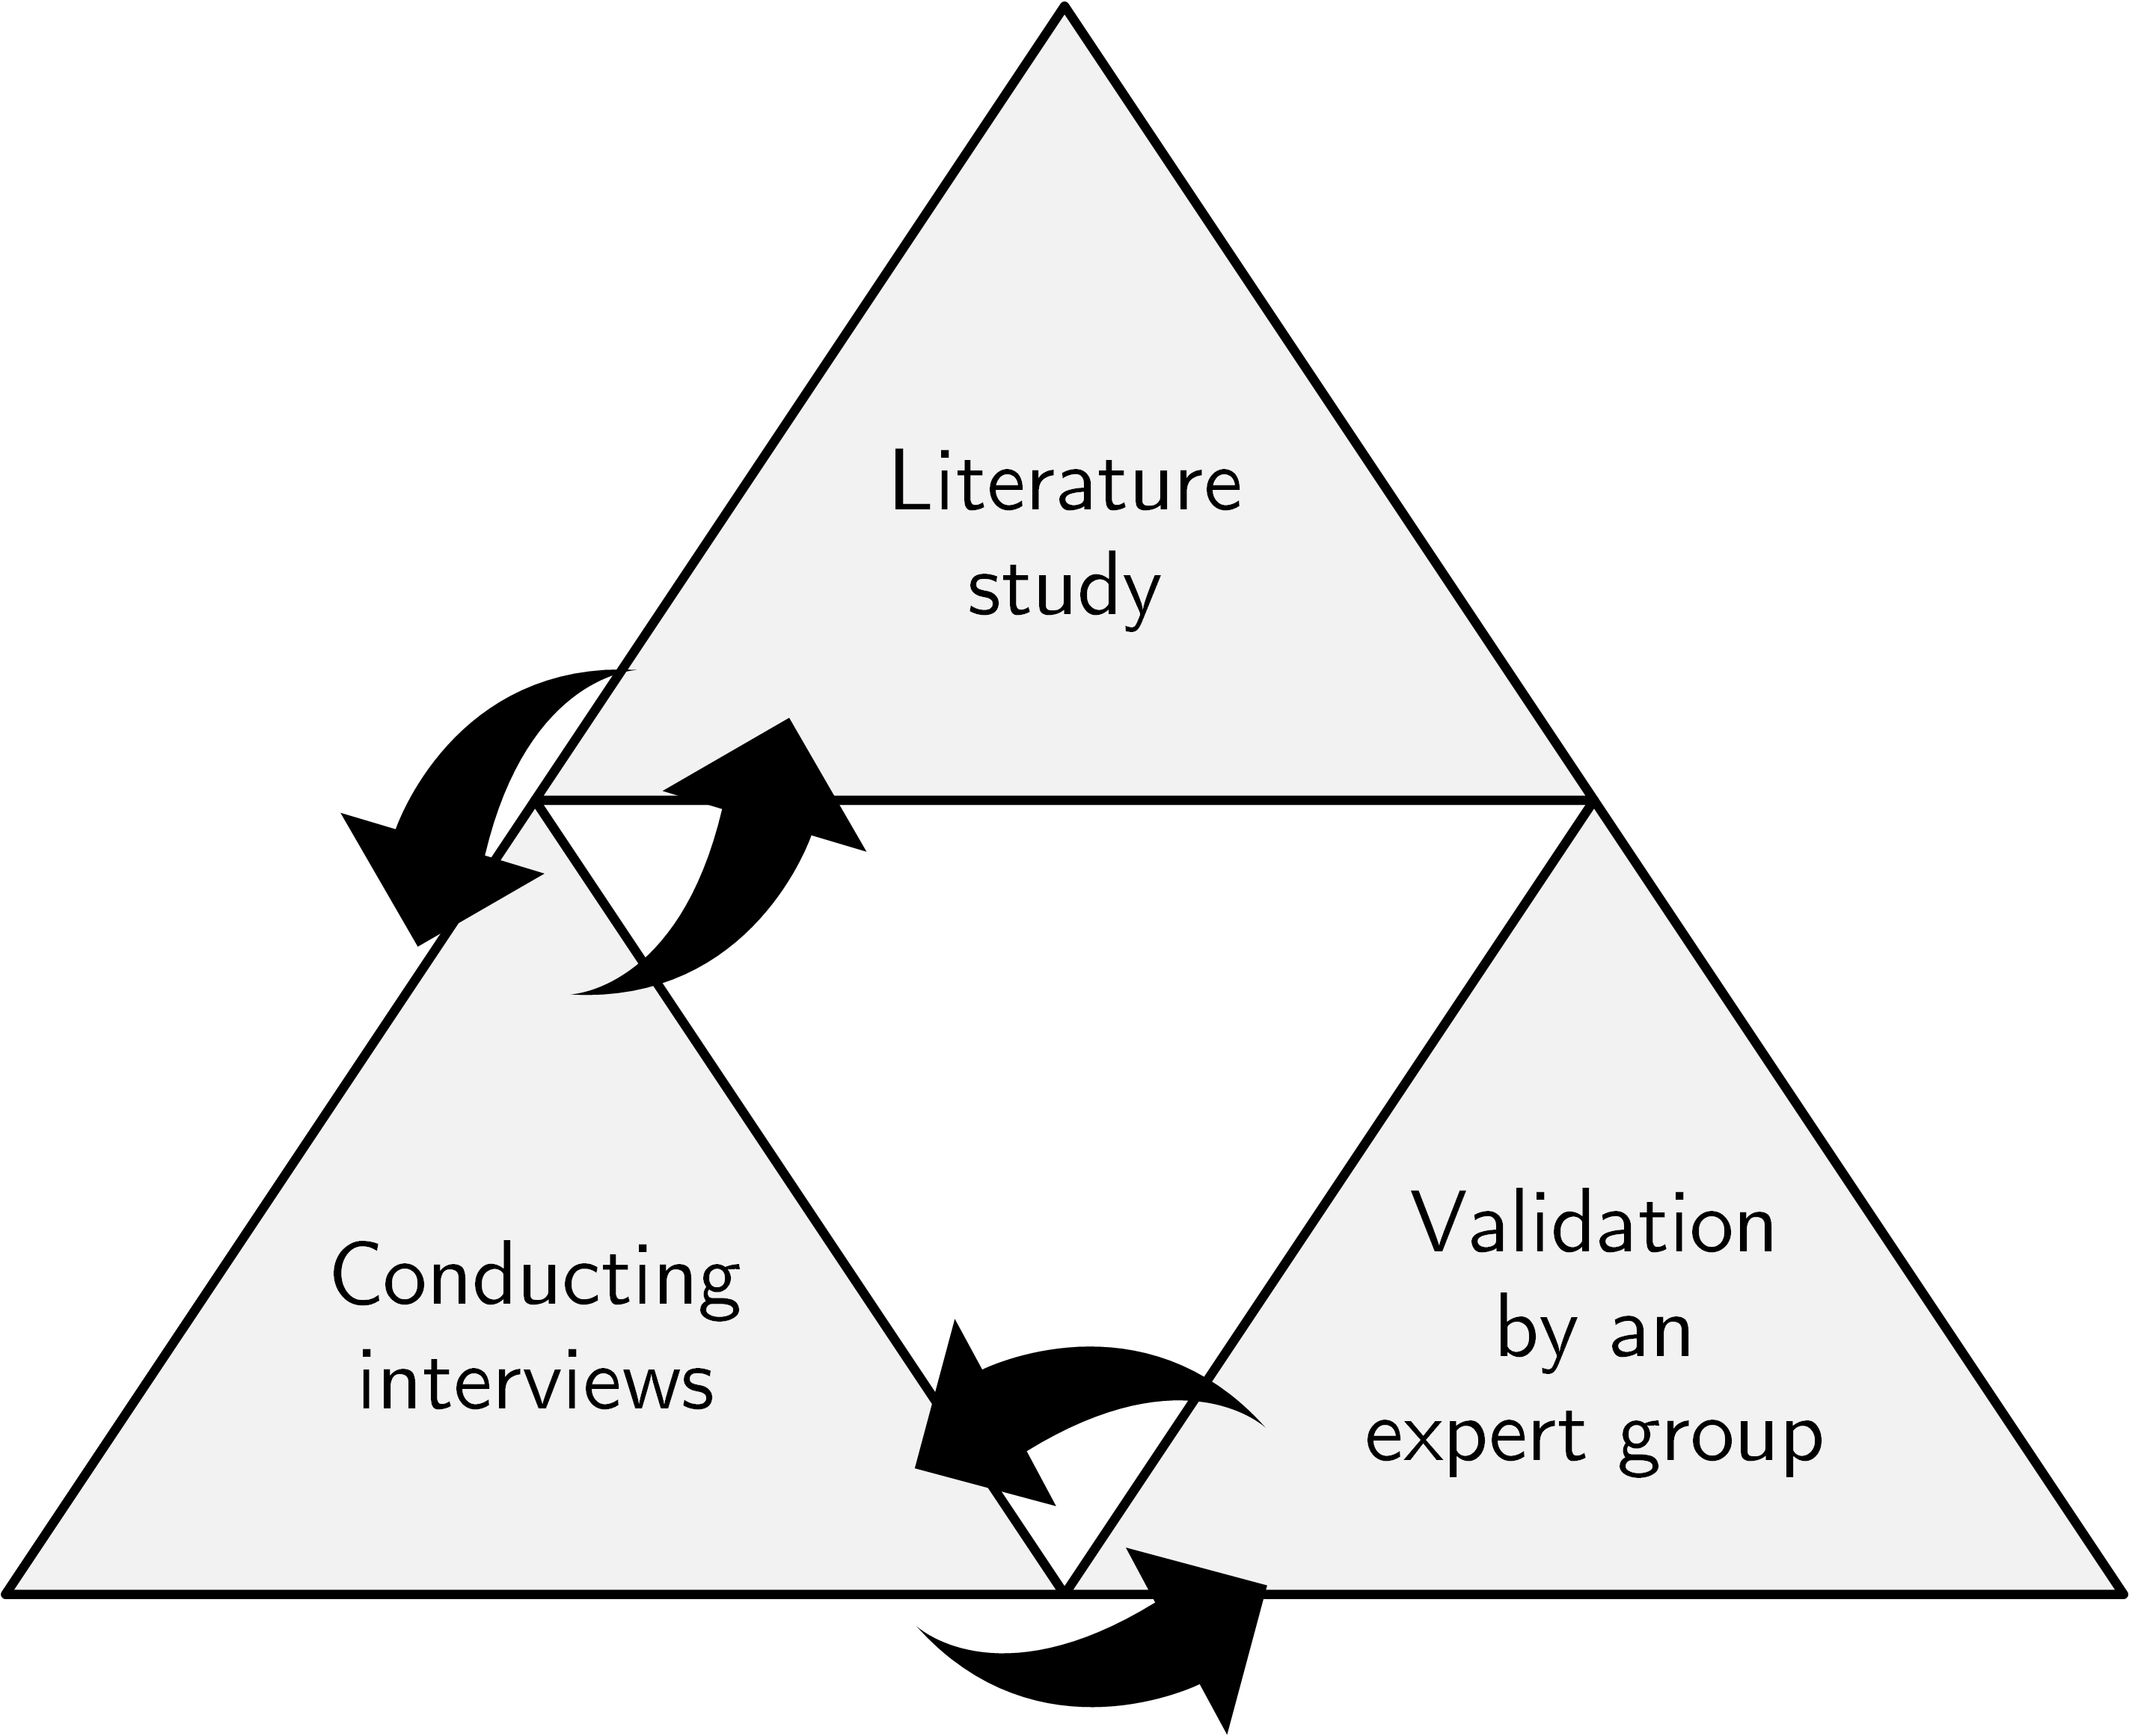
\includegraphics[width=0.45\linewidth]{images/researchmodel}
	\caption[Research model]{Research model}
	\label{fig:researchmodel}
\end{figure}

\section{Research approach}
\label{sec:researchapproach}
How will we conduct the literature study, interviews, and the validation with an expert group? This question is what this section will answer. This section describes the approach in detail to make the research replicable.
\subsection{Literature study}
\label{sub:literaturestudy}
The literature study will answer the first five sub-questions of this research \cref{sec:introresearchquestion}. \Cref{ch:theoreticalbackground} contains the outcome of the literature research. The literature research is conducted by searching literature by using keywords. We use online scientific libraries like Web of Science, Research Gate, Google Scholar, and Semantic Scholar to find relevant literature. We use the full name and the abbreviation of the concept to search for literature. E.g. \acrlong{ea} and \acrshort{ea}. Literature is accepted if it complies with quality \glspl{attribute}. These quality \glspl{attribute} are accuracy, authority, objectivity, currency and coverage\footnote{\url{https://libguides.library.cityu.edu.hk/litreview/evaluating-sources/}}. For replicability and reusability, we administrate the found literature.
\subsubsection{System}
\label{subsub:system}
For snowballing, we use two key literature sources for the system concept. These two sources are \textcites{Ackoff1973}{Gharajedaghi2011}. \textcite{Gharajedaghi2011} is one of the authors recognised by \textcite{Lapalme2012} as a follower of the \acrlong{ea} school of thought of \gls{enterpriseecologicaladaptation} We use the following keywords for the online scientific libraries: \textit{system}, \textit{\acrlong{sos}}, \textit{\acrlong{sie}}, \textit{ecosystem}, \textit{\gls{antifragile} system}, and \textit{\acrlong{ea} system}.
\subsubsection{Antifragile}
\label{subsub:antifragile}
For snowballing, we use two key literature sources for the \gls{antifragile} concept. These two sources are \textcites{Taleb2012}{Botjes2020}. \textcite{Taleb2012} is the author who coined the concept of \gls{antifragile} while \textcite{Botjes2020} conducted extensive literature research on \gls{antifragility}.We use the following keywords for the online scientific libraries: \gls{antifragile}, \gls{antifragile} \gls{robust} \gls{resilient}, \gls{antifragile} \acrlong{ea}, \gls{antifragile} \gls{ps}, \gls{antifragile} success factor, \gls{antifragile} system.
\subsubsection{Enterprise Architecture}
\label{subsub:enterprisearchitecture}
We use six key literature sources for the \acrlong{ea} concept for snowballing. These six sources are from authors who align with the \acrlong{ea} school of thought of \gls{enterpriseecologicaladaptation} (\cref{tab:eeaauthors}). The six sources are \textcites{Martin1995}{Graves2008}{Hoogervorst2009}{Gharajedaghi2011}{Smith2011}{Lapalme2012b}. We use the following keywords for the online scientific libraries: \acrlong{ea}, \acrlong{ea} success factors, \acrlong{ea} \gls{antifragile} system, \acrlong{ea} ecosystem, \acrlong{ea} \gls{ps}, \acrlong{ea} \acrlong{sie}, \acrlong{ea} \acrlong{sos}.
\subsubsection{Public sector}
\label{subsub:publicsector}
We use two key literature sources for the public sector concept for snowballing. These two sources are \textcites{Wal2008}{Nurmi2021}. \textcite{Wal2008} compares the public and private sectors on core values while \textcite{Nurmi2021} researches the use of ecosystems in the public sector. We use the following keywords for the online scientific libraries: \gls{ps}, \gls{ps} \gls{antifragile}, \gls{ps} \gls{resilient}, \gls{ps} system, \gls{ps} ecosystem, \gls{ps} \acrlong{sos}, \gls{ps} \acrlong{sie}, \gls{ps} collaboration with the private sector, and \gls{ps} differences to the private sector.
\subsection{Interviews}
\label{sub:interviews}
The interviews are in the format of semi-structured. A minimal set of questions is used because of time constraints. The set of questions is created by combining multiple attributes into one question. A \gls{conceptmap} is created to define which question will give a possible answer to what attribute. The \gls{conceptmap} is appended to the thesis, see \cref{app:cmapinterviewattributes}. Based on given answers, there will be further elaboration on the topic when there is a suspicion of extra information about \acrshort{ea} and \gls{antifragile} attributes. The interviews are recorded and transcribed. The transcriptions will be summarised and appended to this thesis, see \cref{app:interviewsummaries}. The transcriptions will be labeled with the earlier found attributes, \cref{sub:literaturestudy}, so that analysis can take place in a numerical form. The labeling will be done with a positive and a negative label. E.g. \textit{Antifragile} and \textit{Not Antifragile}. If the attribute is mentioned with a question per interview, it will only be counted once for that question for that interview. When an attribute is at least mentioned in 75\% of the interviews (cases) and the sum of the positive and negatives labels is equal or lower than 0 it could be a success factor. Newly found attributes are scored in the same way.
\subsection{Expert Group}
\label{sub:expertgroup}
The Expert Group is used to validate the findings from the interviews. Because the interviews already validated the initially found attributes the Expert Group will validate these for a second time. These findings are a subset of the original set found in the literature. The Expert Group is carefully composed of \acrshort{ea} specialists from the \gls{ps} with a balance between the governments and privately-held companies, all part of the public sector or \acrshort{ea} specialists with recent experience with the \gls{ps}. For the validation by the Expert Group, a meeting will be planned. All the known definitions and the agenda are shared with the Expert Group for preparation. The Group Support System Meeting Wizard supports this meeting. A presentation is used to bring the participants up to speed on the status of the research. Meeting Wizard will facilitate brainstorming for possible missed attributes, ordering the attributes and voting on the attributes. Meeting Wizard will also support surveys to determine the experience in \acrshort{ea} and the \gls{ps} and the relevance of the research. The output from the Expert Group will be analysed in the same way and with the same rules as that of the interviews. Everything must be normalised and be transformed into numeric values. The outcome of the Expert Group Validation will also trigger a second round of labelling the interviews for the new findings. 
\subsection{Analysis}
\label{sub:analysis}
By combining the outcomes from the literature study, the interviews, and the Expert Group, a list of attributes is made with attributes that are most likely to be success factors. For the analysis, \gls{triangulation} is used. It will be plausible for the research data set that the attribute is a success factor if it meets three requirements. The first requirement is that the attribute was found in the literature. The second requirement is that the attribute was confirmed with interviews. The last requirement is that the Expert Group agreed on the attribute as a possible success factor. This step in the research will answer the sub-question ''Which success factors can positively influence the contribution of \acrlong{ea} in achieving \gls{antifragility} in the \gls{ps}?''
\subsection{Conclusion and discussions}
\label{sub:conclusionanddiscussions}
This chapter will give a definitive answer to the research question ''What are the success factors that positively influence the contribution of \acrlong{ea} in achieving \gls{antifragility} in the \gls{ps}?'' This chapter states the found and validated attributes as possible success factors for the data set that was used for the research. The chapter also contains a discussion on falsification and other findings.

\section{Research infrastructure and tooling}
\label{sec:researchinfraandtooling}
For selecting the suitable instruments for the research, the Open Science Framework\footnote{\url{https://www.cos.io/products/osf}} is used, see \cref{fig:openscienceframework}. The Open Science Framework proposes specific infrastructure and tools per stage. The transparency in the used infrastructure and tools increases the quality of the research by increasing replicability, findability, accessibility, interoperability, and reusability.
\subsection{Research execution}
\label{sub:tbresearchexecution}
For the execution of the research, Microsoft Excel\footnote{\url{https://www.microsoft.com/en-us/microsoft-365/excel}} is used for the administration of the literature research. For the administration of the literature research, the following headers are used: ID (for a unique ID per item), search terms used, scope, title, subtitle, author(s), year, type, Bib\LaTeX\ citation key, title relevance, abstract relevance, content relevance, found at, doi/isbn, url, date found, duplicate, date used, use for, and notes. Researchgate\footnote{\url{https://www.researchgate.net/}}, Web of Science\footnote{\url{https://app.webofknowledge.com/}}, Google Scholar\footnote{\url{https://scholar.google.com/}}, and Semantic Scholar\footnote{\url{https://www.semanticscholar.org/}} are the main sources for searching for literature. PaperPanda\footnote{\url{https://paperpanda.app/}} is used for hard to find literature. The literature administration is, together with the publicly available literature, stored in the repository of the master thesis\footnote{\url{https://github.com/JRBliekendaal/master-thesis/tree/main/literature}}. For non-public available literature, the administration contains the location where the literature is retrievable. All the literature is added to a bib\LaTeX\ file for future reference. For traceability the entries in the bib\LaTeX\ file contain the Unique ID in the notes field. The references are sorted into subgroups. The subgroups used are: ''evaluate, rejected, and used.'' Only the literature in the subgroup used are transferred to the bibliography file of the thesis. For working as paperless as possible all the literature, is in pdf or in ebook format. For reading Acrobat Reader DC\footnote{\url{https://get.adobe.com/reader/}} is used for reading the PDF, and an Amazon Kindle Oasis\footnote{\url{https://www.amazon.com/dp/B07L5GJD99}} for eBooks. With the Amazon Kindle the highlight feature is used. This is not stored on GitHub since the highlights are under copyright of the author(s). For interviews Microsoft Teams is used with the transcript and session recording functionality. The transcript is full of sensitive information and is not publicly available. To make sure that the necessary information is available summaries are created and added to the thesis. The recordings are securely stored and are available upon request by the Antwerp Management School. The transcripts are used in QDA Minder Lite\footnote{\url{https://provalisresearch.com/products/qualitative-data-analysis-software/freeware/}} to label the interviews so that analysis can be done with Microsoft Excel. For the Expert Group, Meetingwizard\footnote{\url{https://www.meetingwizard.nl/}} is used for brainstorming, surveys and voting. The license for using Meeting Wizard is supplied by the Antwerp Management School. The output of the Meeting Wizard session is stored as a Microsoft Excel file in the repository of the thesis (anonymised).
\subsection{Research administration}
\label{sub:tbresearchadministration}
The research administration, which includes documentation containing privacy-sensitive information, like the name and contact information of the Expert Group participants, is stored on a non-public GitHub Repository\footnote{\url{https://github.com/JRBliekendaal/master-thesis-administration}}. The private GitHub Repository is also for staging thesis parts that still need to be anonymised. For taking notes Leuchtturm1917\footnote{\url{https://www.leuchtturm1917.us/notebook-classic.html}} Notebooks are used a mechanical pencil of Rotring\footnote{\url{https://www.rotring.com/pens-pencils/pencils/rotring-600-mechanical-pencil-1/SAP_1904443.html}}.
\subsection{Thesis creation}
\label{sub:tbresearchcreation}
I used my Apple MacBook Air M1 for creating the thesis. The thesis is created with the markup language \LaTeX\footnote{\url{https://www.latex-project.org/}}. The used typesetting environment is MacTex\footnote{\url{https://www.tug.org/mactex/}} with the document type of ''Report'' from KOMA-Script\footnote{\url{https://ctan.org/pkg/koma-script}}. TexStudio\footnote{\url{https://www.texstudio.org/}} is the used \LaTeX\ Editor. It supports syntax-highlighting, has an integrated viewer, reference checking and numerous wizards. For the creation and administration of references Bib\LaTeX\footnote{\url{https://ctan.org/pkg/biblatex/}} is used with the citation style of APA 7th Edition\footnote{\url{https://apastyle.apa.org/}}. The files are stored on a Apple iCloud\footnote{\url{https://www.icloud.com/}} that is used by GitHub Desktop\footnote{\url{https://desktop.github.com/}} to synchronise with a public GitHub repository\footnote{\url{https://github.com/JRBliekendaal/master-thesis}}. GitHub\footnote{\url{https://github.com/}} is used for source control but also for reviewing and discussing the topics with my (Co-)Promotor and the planning of the master thesis project. The thesis source files are copied to an Amazon S3 Blob\footnote{\url{https://aws.amazon.com/s3/}} for backup. The backup rotation is seven versions. Cloudberry Explorer Freeware for Amazon S3\footnote{\url{https://www.msp360.com/explorer/windows/amazon-s3.aspx}} is used for backup. Grammarly\footnote{\url{https://www.grammarly.com}}, with the paid subscription service, checks the thesis for spelling, grammar,  style, and plagiarism. The used goals for Grammarly are audience=knowledgeable, formality=formal, and domain=academic. Microsoft Visio Professional\footnote{\url{https://www.microsoft.com/en-ww/microsoft-365/visio/}} is used to create figures. The GitHub repository contains all the sources\footnote{\url{https://github.com/JRBliekendaal/master-thesis/tree/main/images/sources}}.

\section{Research quality implementation}
\label{sec:researchqualityimplementation}
The research model is defined. But how do we ensure that this approach also fulfils our quality requirements? We have two sets of quality principles we want to fulfil. The set of \textcite{Recker2012} and the FAIR principles of \textcite{GOFAIR2017}.

When we look at the principles of \textcite[pp.~15--17]{Recker2012} we have the principles replicability, independence, precision, and falsification. We ensure that the thesis contains a description of all steps. Steps taken for the literature study, the interviews, and the expert group.  To support replicability the used data sets are publicily available for use.

Replicability, independence, precision, and falsification are the principles \parencite[pp.~15--17]{Recker2012}. We ensure that the thesis contains a detailed approach for replication. The used data sets are made publicly available to support replicability. By rationalising everything, we remove as much subjectivity as possible. The output of the interviews and the expert group are normalised to remove possible bias from the system. This approach supports the principle of independence. Defining every concept supports the principle of precision. For every concept, there is a clear definition available. When there are more definitions, research is necessary. Using a rationale makes it clear why we did choose a particular definition. All the definitions are available in \cref{ch:theoreticalbackground} or the Glossary of Terms. Using discussions (\cref{sec:discussions}) helps with the falsification of this research.

Findable, accessible, interoperable, and reusable are the principles of FAIR \parencite{GOFAIR2017}. Keywords, links, structures, and metadata that can be indexed support findability. GitHub, Zenodo, and Researchgate publish the thesis and the used data sets. We created objects with a location for acquiring the source for sources that are not to be published publicly. Publishing based on Open Access supports the principle of accessibility. The principle that is least relevant for this research is interoperable. It is least relevant because this principle is mostly for quantitative methods. Nevertheless, the datasets are available as Microsoft Excel files for analysis. The files are easy to import, reuse, or combine in other environments to support the principle of reusability. The publication of the thesis and the used datasets use a Creative Commons license (\href{https://creativecommons.org/licenses/by-sa/4.0/}{CC-BY-SA 4.0}). The thesis and the used data sets can be shared and adapted as long as the original author is attributed and the possible derivate uses the same license.



